\documentclass[10pt]{article}
\usepackage[margin=1in, paperwidth=8.5in, paperheight=11in]{geometry}
\usepackage{ifpdf,amsmath, amssymb, comment, color, graphicx, stmaryrd,setspace,enumitem,tikz, fancyhdr, wrapfig, textcomp, units, mathptmx, pdfpages, cancel, multicol}
\usepackage{hyperref}
\hypersetup{
    colorlinks=true,
    urlcolor=blue,
}

\setlength{\headheight}{14.5pt}
\newcommand{\Q}{\mathbb{Q}}
\newcommand{\R}{\mathbb{R}}
\newcommand{\Z}{\mathbb{Z}}
\newcommand{\vu}{\mathbf{u}}
\newcommand{\vv}{\mathbf{v}}
\newcommand{\vw}{\mathbf{w}}
\newcommand{\vi}{\mathbf{i}}
\newcommand{\vj}{\mathbf{j}}
\newcommand{\vk}{\mathbf{k}}
\newcommand{\vn}{\mathbf{n}}
\newcommand{\vr}{\mathbf{r}}
\newcommand{\va}{\mathbf{a}}
\newcommand{\vF}{\mathbf{F}}
\newcommand{\vL}{\mathbf{L}}
\newcommand{\vT}{\mathbf{T}}
\newcommand{\vN}{\mathbf{N}}
\newcommand{\proj}{\operatorname{proj}}
\newcommand{\orth}{\operatorname{orth}}
\newcommand\del\nabla
\newcommand\dotp[1][.5]{\,\mathbin{\vcenter{\hbox{\scalebox{#1}{$\bullet$}}}}\,}
\newcommand{\slice}{_\text{slice}}

% Solution text is in red. If you want the solutions to show, remove the \iffalse from the definition of the \red command.
%\newcommand{\red}[1]{ %\iffalse
%	\textcolor{red}{#1} }%\fi}

\newenvironment{red}{\color{red}}{\ignorespacesafterend}
\newenvironment{blue}{\color{blue}}{\ignorespacesafterend}
\newcommand{\green}[1]{\textcolor{green}{#1}}
\renewcommand{\section}[1]{\begin{center} \textbf{#1} \\\end{center}}
%
\hyphenpenalty=5000
\setlength{\parindent}{0in}
%\oddsidemargin=-.25in
\allowdisplaybreaks
\pagestyle{fancy}
\renewcommand{\headrulewidth}{0pt}
\lhead{MATH 202}
\rhead{Spring 2024}
%\lfoot{\copyright\ CLEAR Calculus 2010}
\cfoot{}

\begin{document}
%


%\onehalfspacing
\allowdisplaybreaks
%##################################################################
\section{PS\#9: Verifying and sketching solutions to DEs - \red{Answer key} }


Consider the differential equation $\displaystyle \frac{dy}{dt} = y-t$.

\begin{enumerate}[leftmargin=0pt]

\item (Modified from \href{https://activecalculus.org/single/sec-7-1-diff-eq-intro.html#mvy}{AC 7.1 Exercise 6}) A magic seashell has whispered into our ear that the following functions might be solutions to the differential equation. However, it is a \textit{rude} magic seashell which sometimes lies. Determine whether each of the following functions is a solution to the differential equation:


\begin{enumerate}
    \item $y(t) = t-2e^t+1$
    
    \begin{red}
    The LHS of the differential equation is $\dfrac{dy}{dt}$, which in this case is $1-2e^t+0$. 
    
    The RHS of the differential equation is $y-t$, which in this case is $\left(t-2e^t+1\right)-t = 1-2e^t$. 
    
    So, this \textbf{is a solution}, yay, because the LHS and the RHS match.
    \end{red}
    \item $y(t) = t+1$
    
    \begin{red}
    The LHS of the differential equation is $\dfrac{dy}{dt}$, which in this case is $1 + 0$. 
    
    The RHS of the differential equation is $y-t$, which in this case is $\left(t+1\right)-t = 1$. 
    
    So, this \textbf{is a solution}, yay, because the LHS and the RHS match.
    \end{red}

    \item $y(t) = 2e^t$

    \begin{red}
    The LHS of the differential equation is $\dfrac{dy}{dt}$, which in this case is $2e^t$. 
    
    The RHS of the differential equation is $y-t$, which in this case is $\left(2e^t\right)-t$. 
    
    So, this \textbf{is not a solution}, boo, because the LHS and the RHS \textbf{don't} match.
    \end{red}
    \item $y(t) = 1+\frac{e^t}{2}+t$
    
    \begin{red}
    The LHS of the differential equation is $\dfrac{dy}{dt}$, which in this case is $0 + \frac{e^t}{2}+1$. 
    
    The RHS of the differential equation is $y-t$, which in this case is $\left(1+\frac{e^t}{2}+t\right)-t = 1+\frac{e^t}{2}$. 
    
    So, this \textbf{is a solution}, yay, because the LHS and the RHS match.
    \end{red}
\end{enumerate}

\item One of the correct solutions in \#1 is the exact solution to the initial value problem $\dfrac{dy}{dt} = y-t$, $y(0) = -1$. Which one, and how can you tell?

\begin{red}
$y(t) = t + 1 - 2e^t$. I can tell because, first of all, it \textbf{is} yes a solution, and secondly, because $y(0) = 0 + 1 - 2e^0 = -1$.
\end{red}
\begin{enumerate}
    \item Bonus question: What $y(0) = \rule{0.7cm}{0.15mm}$ are the other correct solutions?

    \begin{red}
        The other correct solutions are 
        \begin{itemize}
            \item $y(t) = t + 1$, which has $y(0) = 1$,
            \item and $y(t) = 1+\frac{e^t}{2}+t$, which has $y(0) = 1 + \frac12 + 0 = \frac32$.
        \end{itemize}
    \end{red}
\end{enumerate}

Problem set continues on next page.

\pagebreak

\item (Modified from \href{https://activecalculus.org/single/sec-7-2-qualitative.html#OvE}{AC 7.2 Exercise 5}) Now we're going to explore the slope field for $\dfrac{dy}{dt} = y-t$.
\begin{enumerate}
    \item Produce a slope field for this differential equation. You can use \href{https://homepages.bluffton.edu/~nesterd/apps/slopefields.html}{technology} and take a screenshot, or you can generate one by hand; it's up to you. Your slope field should at least show the window $-3\leq y \leq 3$, $-4\leq t \leq 4$.
    \item Sketch the solutions whose initial values are $y(0) = -3$, $y(0) = -2$, and so on up to $y(0) = 3$.
    
    \begin{center}
        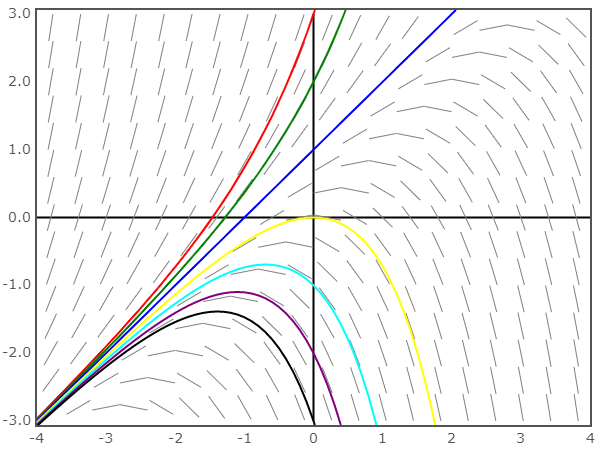
\includegraphics[width=0.8\textwidth]{images/y-t-slopefield.png}
    \end{center}
    \item What do your sketches suggest is the solution whose initial value is $y(0) = 1$? How does this connect to your work on problem \#2?
    
    \begin{red}
    It looks like this solution is linear, and indeed, the solution in \#2(b) was the linear function $y(t) = t+1$.
    \end{red}
    \item Draw a graph of the function $y(t) = t+1-2e^t$ from problem \#1. What's $y(0)$ for this function? How does this graph compare to the sketches you've made?
    
    \begin{red}
    $y(0) = 0+1-2e^0 = -1$, and indeed, the graph of this function matches the sketch I made of the solution whose initial value is $y(0) = -1$. (That's an annoying very light blue in the picture above.)
    \end{red}
    \item (Bonus question) Look at the points where each of these solutions has a local maximum. Notice anything interesting?

    \begin{minipage}{0.6\textwidth}    
    \begin{red}
    If the solution has a local maximum, then $\dfrac{dy}{dt}$ should be 0. So, since $\dfrac{dy}{dt} = y-t$, we can insist that $0 = y-t$ -- in other words, $y=t$. And indeed, if you draw the line $y=t$, which I've done in an annoying magenta color below, it goes smack dab through all of the local maxima of the solutions, including a bunch more that I added for illustration. (Neat! This is called the ``nullcline''.)
    \end{red}
    \end{minipage}
    \hfill
    \begin{minipage}{0.3\textwidth}
        \begin{center}
        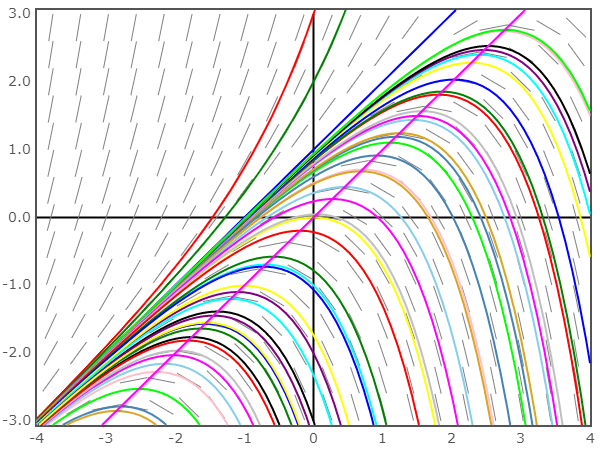
\includegraphics[width=\textwidth]{images/y-t-slopefield-maxes.png}
    \end{center}
    \end{minipage}
\end{enumerate}


\end{enumerate}
\end{document}